\documentclass[10pt,letterpaper]{article}

\usepackage{cogsci}
\usepackage{pslatex}
\usepackage{apacite}
\usepackage{graphicx}
\usepackage{amsmath}
\usepackage{amsfonts}
\AtBeginDocument{\RequirePackage{lmodern, times}}

\newcommand{\argmax}[1]{\underset{#1}{\text{argmax}}\ }

\title{One-shot learning of generative speech concepts}
 
\author{Authors}
 
%\author{{\large \bf Morton Ann Gernsbacher (MAG@Macc.Wisc.Edu)} \\
%  Department of Psychology, 1202 W. Johnson Street \\
%  Madison, WI 53706 USA
%  \AND {\large \bf Sharon J. Derry (SDJ@Macc.Wisc.Edu)} \\
%  Department of Educational Psychology, 1025 W. Johnson Street \\
%  Madison, WI 53706 USA}

\begin{document}
\maketitle

\begin{abstract}
\textbf{Keywords:}
speech recognition; category learning; one-shot learning; exemplar generation
\end{abstract}

\section{Introduction}
There has been recent interest in one-shot learning -- the human ability to learn a new concept from just one or a few examples \cite<e.g.,>{CareyBartlett1978,Markman1989,Ahn1992,Xu2007}. Although one-shot learning is an important aspect of everyday cognition, traditional learning algorithms can require tens, hundreds, or thousands of examples before reaching a high level of classification performance. This mismatch poses a challenge to computational approaches for understanding human-level concept learning, yet over the last several decades, the fields of cognitive science and machine learning have made significant progress. Cognitive models have sought to quantitatively explain the way people generalize from just just a few examples in a low-dimensional space \cite{Shepard1987,Feldman1997,Tenenbaum2001}. Other cognitive models and computer vision algorithms become better one-shot learners through ``transfer learning'' or ``learning to learn,'' where previous experience with related concepts helps to inform which dimensions or features are most important for generalization \cite{Bart2005,Colunga2005,FeiFeiFergus2006,KempPerfors2007}.

Despite real progress spanning multiple disciplines, we are still far from a satisfying computational account of one-shot learning. Previous models have been limited by the simplicity of the representations that they learn -- usually prototypes or exemplars in a feature space -- which lack the power necessary for capturing many types of natural concepts \cite{Murphy1985}. While these feature-based approaches can be useful for classification, they provide less insight into how background knowledge interacts with learning or how people generalize in other ways beyond classification, including exemplar generation \cite{Jern2013}, causal inference \cite{Rehder2003}, explanation \cite{Williams2010}, and conceptual combination \cite{Murphy1988}. Given that people learn very rich concepts, even from just one or a few examples, the central computational challenge is to explain how people extract so much information from such limited data.

Analysis-by-synthesis is the classic idea, beginning with Helmholtz, that sensory data can be more richly represented by modeling the causal process that generates it. This has been an influential approach to studying perception in vision \cite{Yuille2006} and speech \cite{Liberman1967}, where a perceptual classification decision can be made by selecting the category $c \in \{1,...,K\}$, defined by parameters $\psi_c$, that maximizes the probability of generating a data example $x^{(i)}$
\begin{equation}
\argmax{c} P(x^{(i)}|\psi_c).
\end{equation}
But learning is a more challenging problem, and there are good reasons to think an analysis-by-synthesis approach would not be successful for one-shot concept learning. Learning of a causal process from examples $x^{(1)},...,x^{(n)}$ can be formulated as the selection of a model $\psi_c$
\begin{equation}
\argmax{\psi_c} \prod_{i=1}^{n} P(x^{(i)} |\psi_c) P(\psi_c),
\end{equation}
from a potentially infinite space of possible models. Since this can be a very difficult problem and can require many training examples to achieve good generalization \cite<e.g.,>{Geman1992,HintonNair2006}, how could it possibly be learned from just a single training example? One-shot learning of generative models might only be sensible for a special subset of simple causal processes. If a human or machine was trying to learn what a ``tree'' was from just a single example, it would be hopeless to try to learn (or even represent) a fully-detailed process of biological growth, beginning with tree DNA and ending with the set of all possible trees. But at the right level of abstraction, the essence of a tree could be captured by a simple stochastic program, starting with a single branch and then recursively splitting until the tree terminates. With a prior $P(\psi_c)$ favoring simple generative processes, it seems possible to discover such a program from just a few examples.

What is the right notion of simplicity for formulating a prior over causal processes? Recent behavioral and computational work suggests that \emph{compositionality} may be key principle for both encouraging representational simplicity and transferring previously learned knowledge from related concepts \cite{Lake2012,Lake2013}. Freely combining primitive structure can be a powerful way to build complex object representations \cite{Biederman1987}, and when combined with ideas from Hierarchical Bayesian modeling \cite{Gelman2004}, it can also be a similarly powerful way to build a ``generative model for generative models'' that can perform one-shot learning. This idea was applied to the one-shot learning of handwritten character \cite{Lake2013}. Given a raw image of a new character, such as a character from a foreign alphabet, the model learns to represent it by a latent dynamic causal process, composed of pen strokes and their spatial relations (Fig. \ref{models}a). Sharing across characters is accomplished by the re-use of stochastic motor primitives (Fig. \ref{models}a-i) that can combine in new ways to make new characters (Fig. \ref{models}a-iv). From just a single example, this model could both classify and generate new  examples at a human level of performance.

\begin{figure*}[t]
\centering
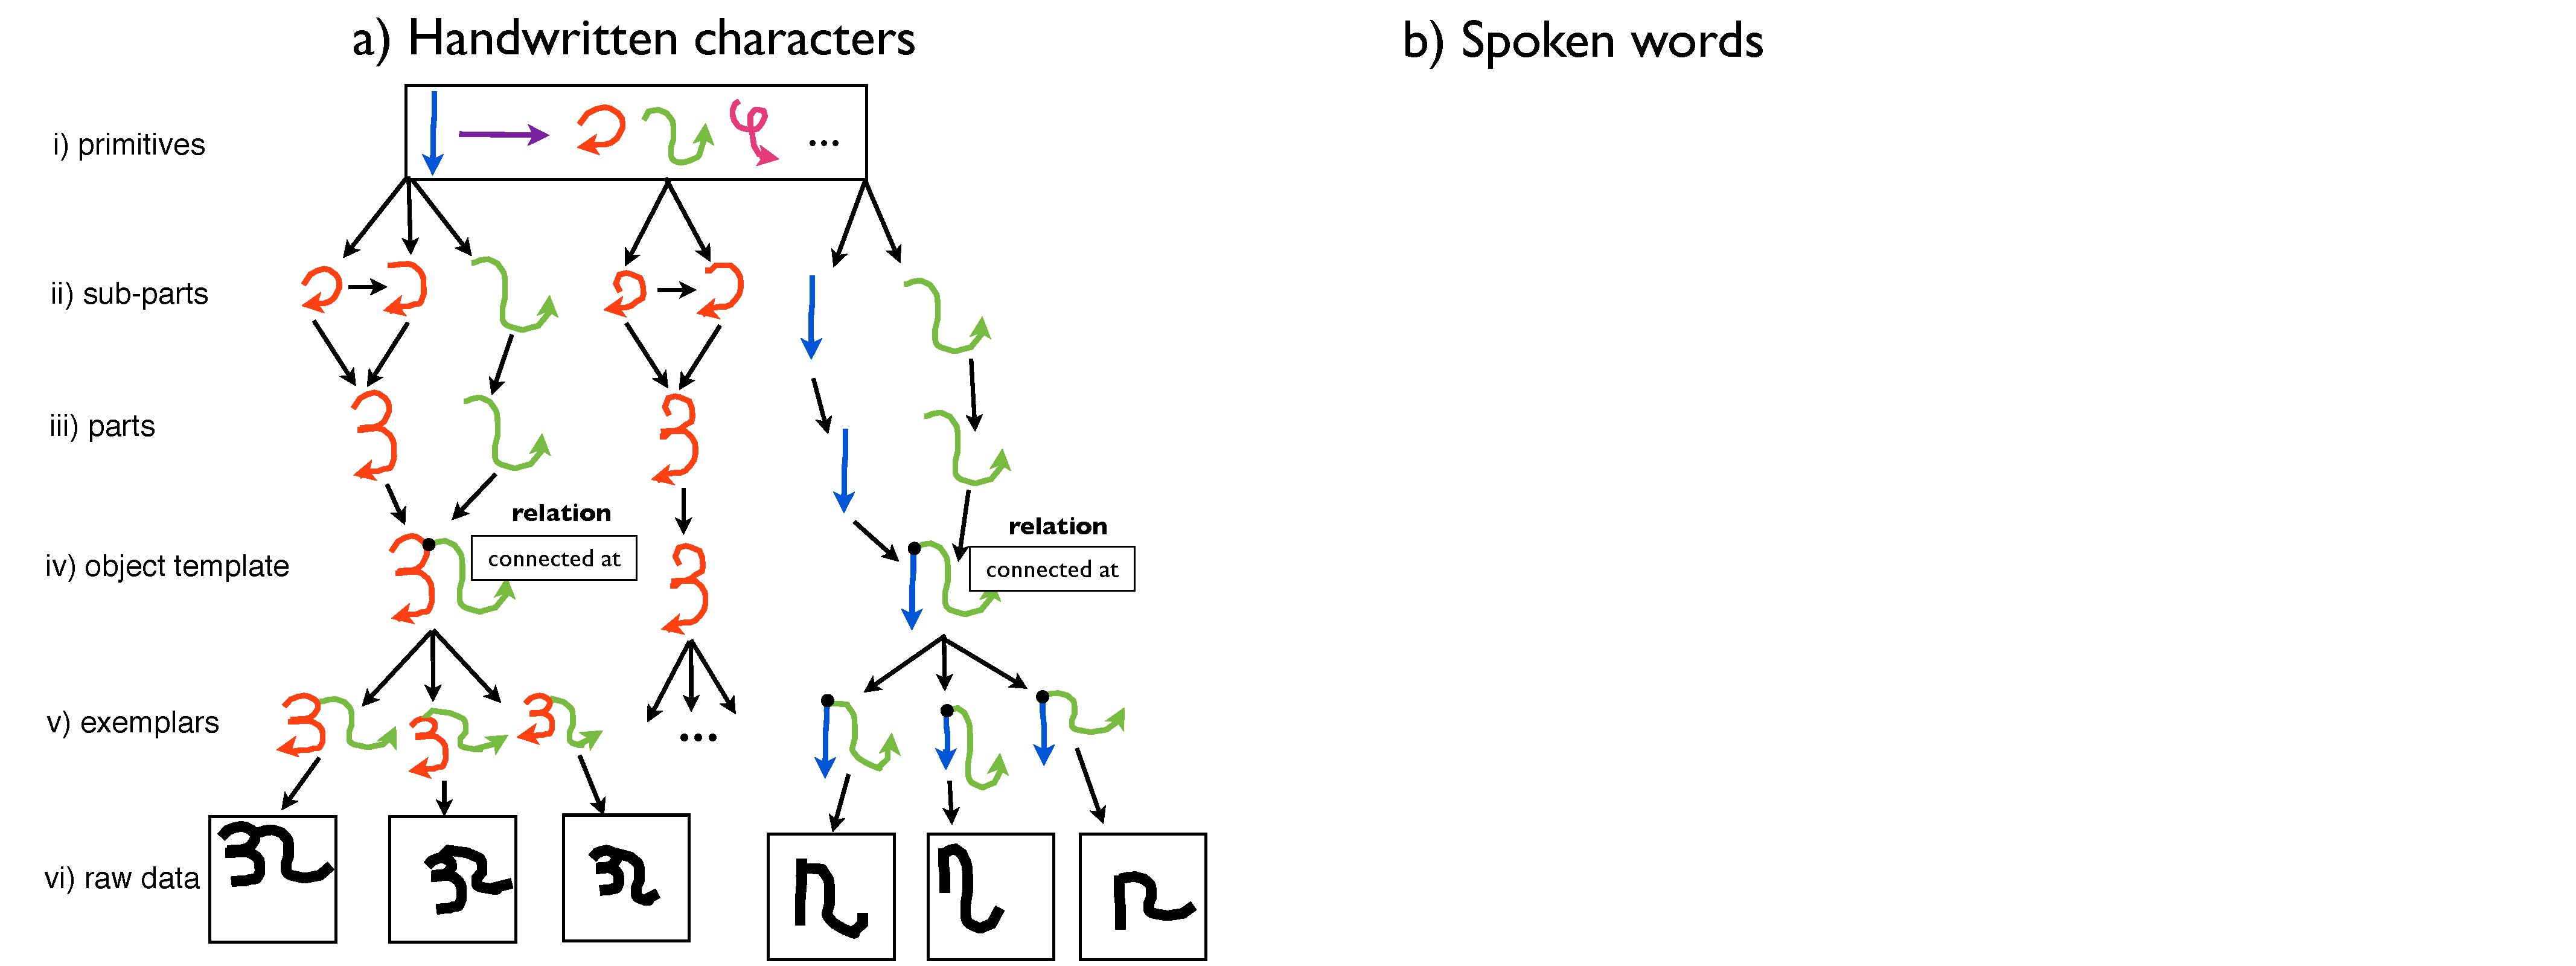
\includegraphics[width=7in]{model.pdf}
\caption{Hierarchical Bayesian modeling as applied to handwritten characters and speech.}
\label{models}
\end{figure*}

How general is this approach, and could it apply to learning non-visual concepts? In this paper, we extend these ideas to the one-shot learning of new spoken words, such as a young child learning to recognize and pronounce a new word (the speech sound for ``elephant'') or an adult learning a word in a foreign language (like the word ``elephant'' in Japanese). Speech is a promising domain for our approach, since analysis-by-synthesis has been influential in speech recognition for decades \cite{Halle1962,Liberman1967} and there is a clear compositional structure of phonemes that could be exploited for learning. From the raw speech signal of a word, our model infers a causal representation based on a sequence of phone-like units (Fig. \ref{models}b). Like the characters, the prior distribution on these sequences are learned from experience with other words and can be combined together in new ways to define a new word (Fig. \ref{models}b-iv). Since each inferred word representation is itself generative, it can be used to both classify new examples or generate new examples (Fig. \ref{models}a-v) from just a single instance of a new word. By transferring a prior on sub-unit sequences learned from a corpus of Japanese speech, the model can classify new Japanese words at a level of accuracy similar to English-speaking humans. We also compare humans and the model on another natural form of generalization -- an exemplar generation task.

\begin{itemize}
	\item Related work in ASR on open dictionary words
\end{itemize}

\section{Model}

\begin{itemize}
\item Describe general ASR approach, and how this is related (but unsupervised, like a child)
\item Mathematical description of the model
\end{itemize}

\section{Experiment 1: Classification}

One-shot classification (20-way) using Japanese words. Here are factors we are going to manipulate.

\subsubsection{People.}
Participants were recruited on Amazon's Mechanical Turk from a population of individual in the USA. All analyses were restricted to native English speakers that do not know any Japanese, as reported in a post-experiment survey rather than as a qualification for participation. This population was used for this and all other experiments. 

Participants were asked to classify new Japanese words. To do so, they were shown a sequence of displays with a button labeled ``target word'' at the top of each display. Below it was a grid of buttons numbered ``1'' through ``20,'' each with an associated radio button for response selection (and a general ``submit'' button to complete the trial). Participants were told that each button played a sound clip of a Japanese word, and their job was to pick the sound clip that produces the same word as the target word. Sound clips could be played more than once, and responses were not accepted until all buttons had been tried.

\begin{itemize}
\item Mention they never see the same word twice
\item Explain word lengths, etc. here or in stimulus section
\item explain instruction checks
\item could click more than once, designed to minimize memory demands
\item explain two conditions (same vs. different gender)
\end{itemize}

\begin{figure}[h]
\centering
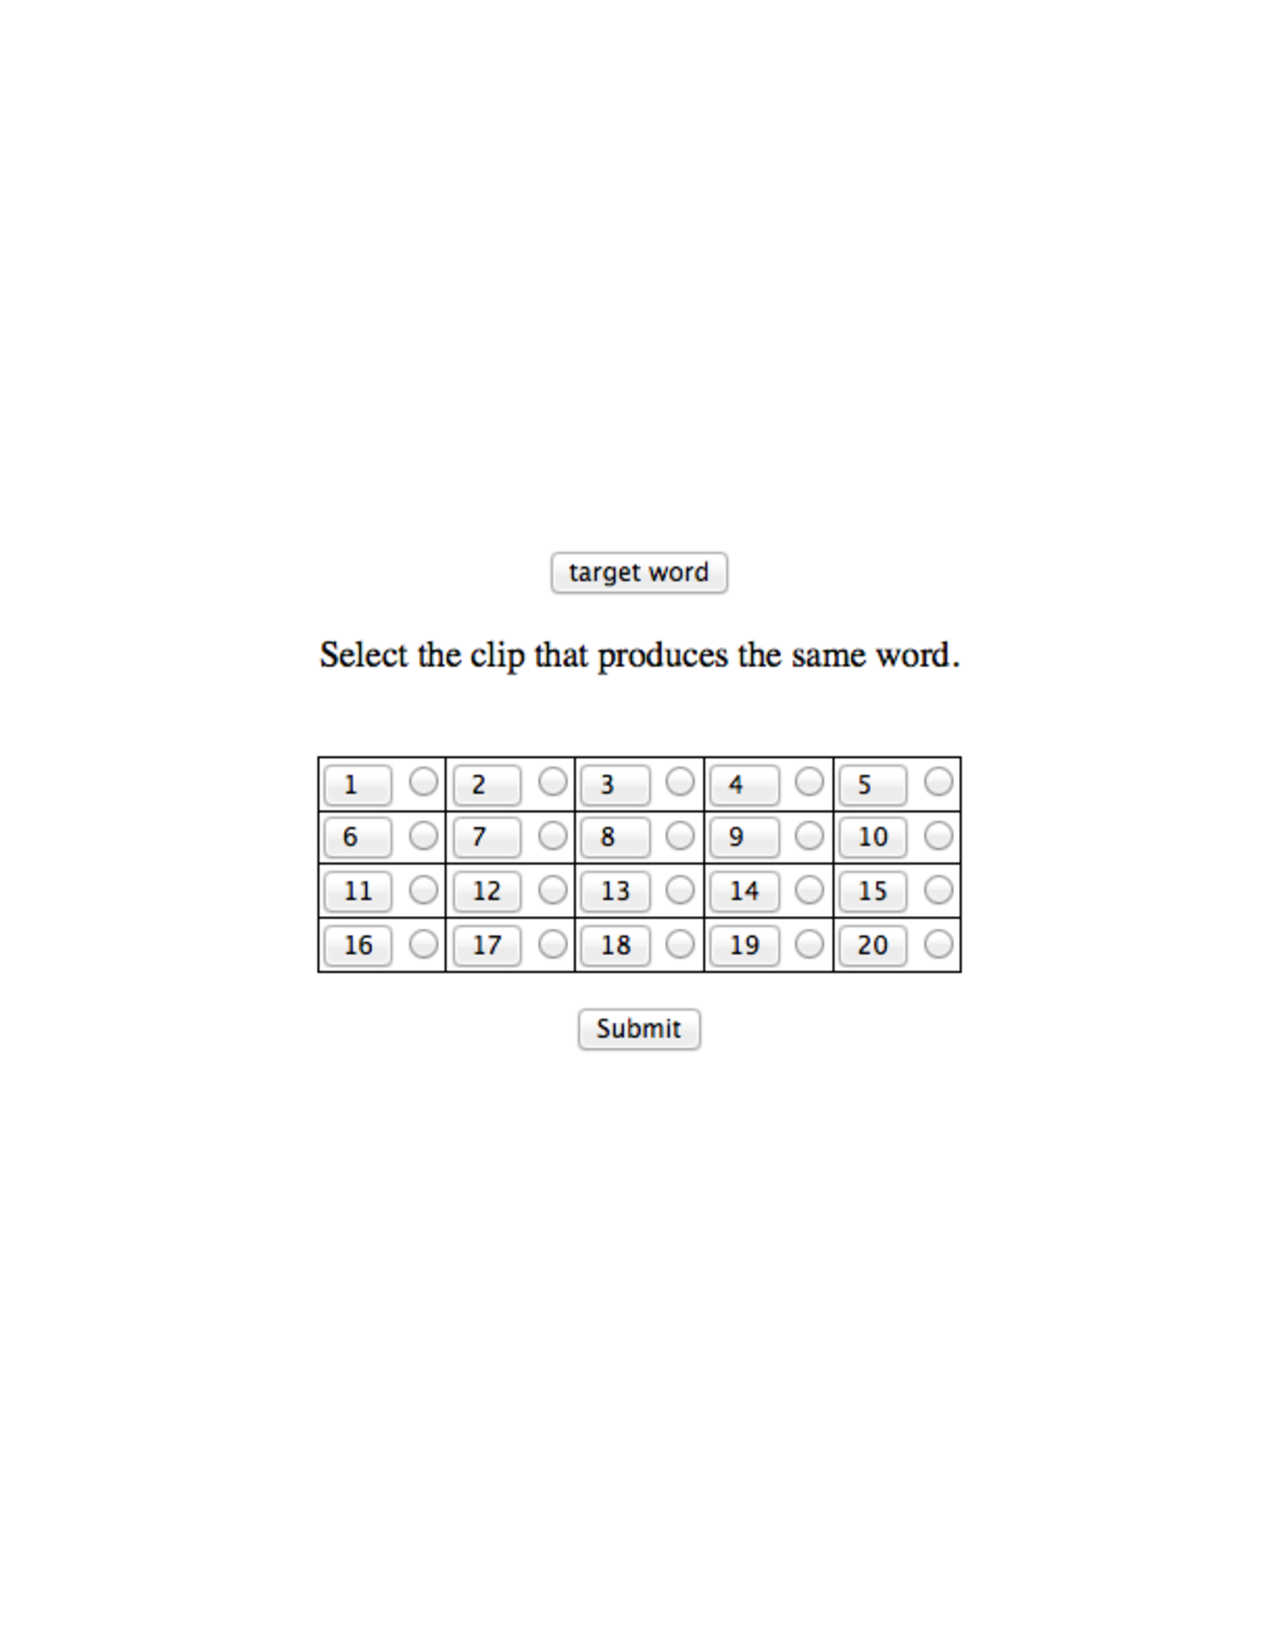
\includegraphics[width=2.25in]{web_exp.pdf}
\caption{Screenshot of web interface for classification judgements. There was also a button to review the full instructions.}
\label{ss}
\end{figure}

\subsubsection{Hierarchical Bayesian model.}

Explain different model conditions and how it makes judgements.
\begin{itemize}
	\item Hierarchical Bayesian (HB) model (trained on English datasets)
	\item HB model (trained on Japanese, using the same corpus and speakers)
\end{itemize}

\subsubsection{Dynamic Time Warp.} 
This is a well-known approach in speech recognition for measure the similarity between two words that requires no learning \cite{Sakoe1978}. Two sequences of feature frames are compared by computing an optimal non-linear warp, using dynamic programming, and then measuring the average distance between the frames of the sequence. 

\subsection{Results}

\section{Experiment 2: Generation}
Classification is just one natural way in which people generalize from one example, and this experiment asked people and various models to generate new examples of a speech concept. Performance was measured by asking other participants to classify the generated examples, providing an indication of whether the new example belongs in the intended class. This is a weaker method for comparing humans and machines than a perceptual ``Turing test,'' as used in our past work with characters \cite{Lake2013}. We did not use this stronger test because our model (and the field of speech synthesis more generally) is not yet up to the task, both in terms of emulating human voice and also in producing a range of different compelling examples instead of just one.

 \subsubsection{People.} Ten participants were asked to say Japanese words after listening to a recording from a male voice. Each participant was assigned a different word length (3 through 12) and then completed twenty trials of speech recording using their computer's microphone. This procedure collected one sample per stimulus used in the previous experiment's classification task. One participant was replaced for very poor recording quality, and another was replaced for knowing some Japanese.

\subsubsection{Hierarchical Bayesian model.}

\begin{itemize}
\item full model (English vs. Japanese)
\item 25\% noise
\item 50\% nosie
\item no primitives
\end{itemize}

\subsubsection{Evaluation procedure.} 
Using a within-subjects design, thirty participants classified a mix of synthesized examples from both people and the comparison models. The trials appeared as they did in Experiment 1 (Fig. \ref{ss}) where the ``target word'' button played a synthesized example. The option clips played original Japanese recordings, matched for word length within a trial as in Experiment 1. Since the synthesized examples were based on male clips, only the female clips were used as options. There was one practice trial (in English) followed by 50 trials with the synthesized example drawn uniformly from the set of all synthesized samples. Since the example sounds vary in quality and some are hardly speech-like, participants were told that the sound quality varies, may be very poor, or may sound machine generated but they were encouraged to try their best. Also, the instructions and practice trial were changed to include a degraded target word clip. All clips were normalized for volume.

\subsection{Results}
Several people commented about the task being too long and too difficult, and two participants were removed for guessing.\footnote{Participants spent between 19 minutes to 87 minutes on the task, and there was also a significant correlation between overall accuracy and time spent (R=0.58, p$<$0.001). In a conservative attempt to eliminate guessing, two participants were removed for failing to listen to the ``target word'' at least twice on per trial on average (6 times was the experiment average). This made little difference for the pattern of results.} The main pattern of results are shown in Fig. \ref{gen_results}. 

\begin{figure}[h]
\centering
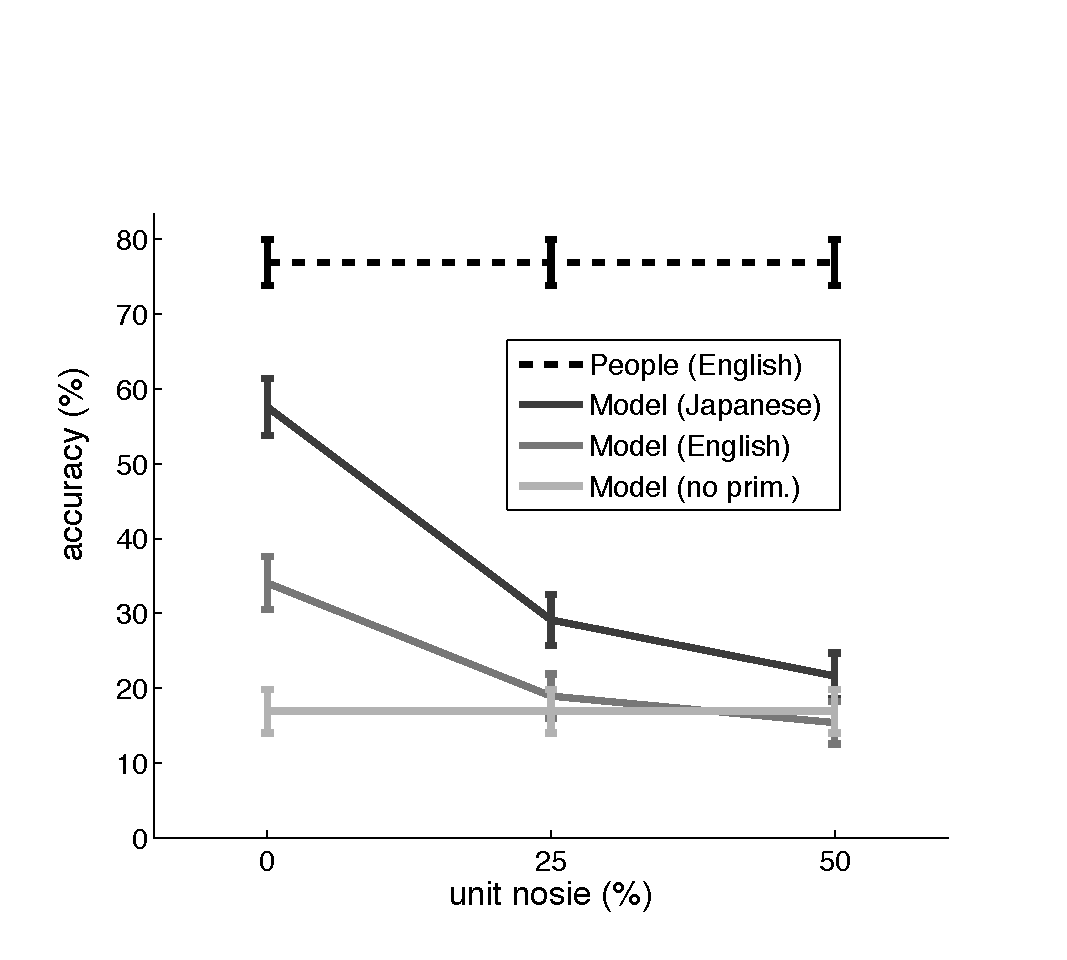
\includegraphics[width=3.25in]{gen_results.pdf}
\caption{Percent of synthesized examples that were identified as belonging to the correct category.}
\label{gen_results}
\end{figure}

\subsection{Replication}
Explain the between subjects replication that we ran here.

\section{Discussion}

\bibliographystyle{apacite}
\setlength{\bibleftmargin}{.125in}
\setlength{\bibindent}{-\bibleftmargin}

\bibliography{library}
\end{document}